\documentclass{report}
\usepackage{fontspec}
\usepackage{polyglossia}
\setdefaultlanguage{french}
\usepackage[a4paper,margin=1.5cm]{geometry}

\usepackage{amsmath}
\usepackage{array}
\usepackage{auto-pst-pdf}
\usepackage{booktabs}
\usepackage{cite}
\usepackage{graphicx}
\usepackage{lmodern}
\usepackage{marvosym}
\usepackage{mathrsfs}
\usepackage{minted}
\usepackage{multicol}
\usepackage{multirow}
\usepackage{paralist}
\usepackage{schemabloc}
\usepackage{siunitx}
\usepackage{soul}
\usepackage{tikz}
\usepackage[european,cuteinductors,siunitx]{circuitikz}
\usepackage{url,hyperref}
\usepackage{verbatim}
\usepackage{xunicode,xltxtra}

\title{
\includegraphics{../../../../../images/inp-enseeiht} \\ ~ \\ ~ \\ ~ \\ ~ \\ Rapport de BÉPO}
\author{Guilhem Saurel}
\date{\oldstylenums{\today}}

\renewcommand{\thesection}{\Roman{section}}

\begin{document}

\begin{titlepage}
    \setcounter{page}{0}
    \maketitle
    \thispagestyle{empty}
\end{titlepage}

\tableofcontents
\newpage



\chapter*{Préambule}
%TODO add it in ToC
\section{BÉPO}
Ceci est mon rapport du Bureau d’Étude de Programation oriente Objet. Il se trouve qu’en en prenant
l’acronyme, on tombe sur BÉPO ; je saute donc sur l’occasion pour glisser un petit lien : \url{bepo.fr}
(vous n’êtes certainement pas sans savoir que l’AZERTY a été conçu pour éviter que les marteaux de 
machine à écrire ne s’entrechoquent… Il est peut être temps d’envisager autre chose). Donc voilà, si,
par hasard, il vous arrive de vous servir d’un clavier, je vous le recommande.

\section{Logiciels utilisés}
Pour la réalisation de ce BÉ et la création de ce rapport, voici une liste non-exhaustives des 
logiciels qui m’ont été les plus utiles:
\begin{description}
    \item[Vim] un éditeur de texte: \url{http://www.vim.org};
    \item[GCC] un compilateur C++: \url{http://gcc.gnu.org};
    \item[git] un gestionnaire de versions: \url{http://git-scm.com/};
    \item[CMake] un moteur de production: \url{http://cmake.org};
    \item[\LaTeX] un logiciel de composition de documents: \url{http://latex-project.org};
    \item[Umbrello] un logiciel de modélisation UML: \url{http://uml.sourceforge.net/};
    \item[GNU Octave] un logiciel de calcul numérique: \url{http://gnu.org/software/octave/};
    \item[ImageMagick] un logiciel de traitement d’images: \url{http://imagemagick.org/script/index.php};
    \item[Bash] un interpréteur de commandes: \url{http://tiswww.case.edu/php/chet/bash/bashtop.html};
\end{description}

\section{UML \& Umbrello}
Umbrello, le logiciel utilisé pour génerer les images présentes dans les différentes sections «UML», utilise
les conventions suivantes:
\begin{itemize}
    \item Trois «cases»: le nom de la classe, les attributs, puis les méthodes;
    \item Les attributs et méthodes «protected» apparaissent avec un «\#», tandis que les «public» utilisent un «+»;
    \item Les variable sont affichées de la manière suivante: «<nom de la variable>: <type de la variable> [<paramètres>]»;
    \item Certaines données ne sont pas affichées, telles que:
        \begin{itemize}
            \item le mot-clef \verb|const|;
            \item le mot-clef \verb|virtual|;
            \item le type \verb|void|;
        \end{itemize}
\end{itemize}

\section{Sources annexes}
Les codes sources du Bureau d’Étude sont naturellement présentes en annexe, mais pour le reste des documents,
tout est disponible sur Github: \url{http://github.com/nim65s/N7/tree/master/be/POO_2A/circuit}, et
notamment le script qui sert à tout (rapport/go.sh).

\chapter{Sources}
    \begin{multicols}{2}
        \section{UML}
            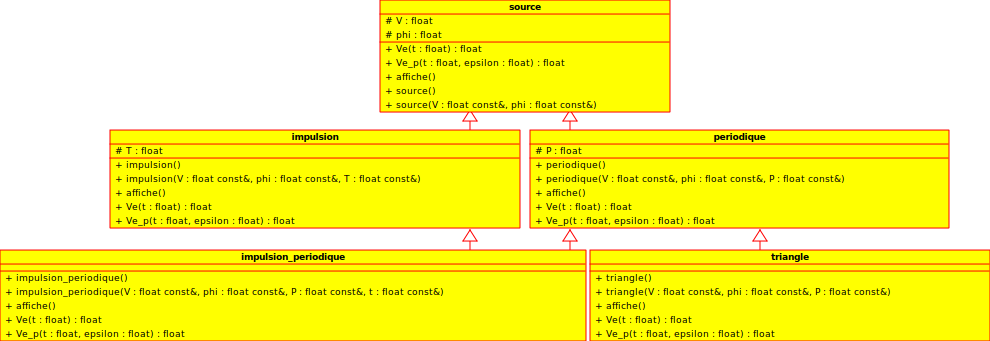
\includegraphics[width=\linewidth+\linewidth,angle=90]{images/sources_large}

        \section{Remarques}
            Ce diagramme UML correspond au fichier «\verb|source.h|».

            La principale difficulté dans ce fichier aura été le «diamant», puisqu’«Impulsion\_periodique» hérite
            d’«Impulsion» et de la classe abstraite «Periodique», ce qui complique un peu les constructeurs.

    \end{multicols}

\chapter{Euler}
    \section{UML}
        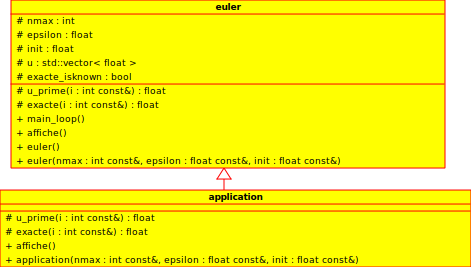
\includegraphics{images/euler_alone}

    \section{Remarques}
        Ce diagramme UML correspond au fichier «\verb|euler.h|».

\chapter{Premier ordre}
    \begin{multicols}{2}
        \section{UML}
            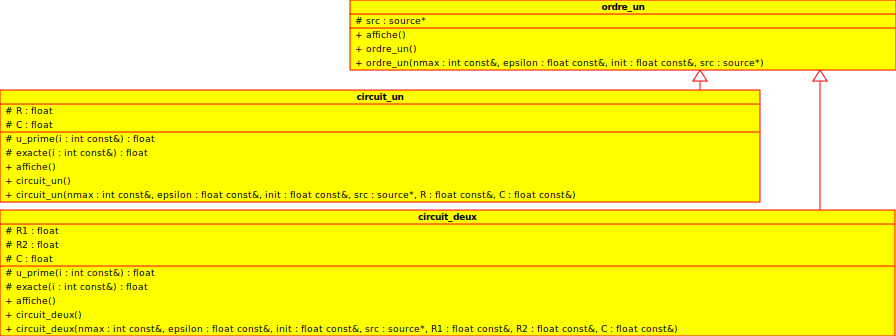
\includegraphics[width=\linewidth+\linewidth,angle=90]{images/ordre_un}

        \section{Remarques}
            Ce diagramme UML correspond au fichier «\verb|ordre_un.h|».

            La classe «ordre\_un» hérite évidemment de la classe «euler», vue dans le chapitre précédent.
    \end{multicols}

\chapter{Second ordre}
    \begin{multicols}{2}
        \section{UML}
            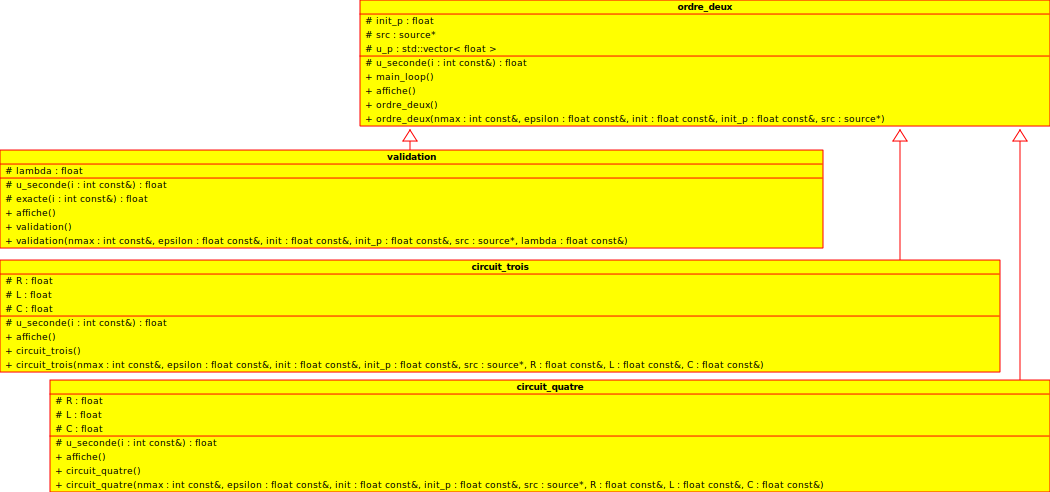
\includegraphics[width=\linewidth+\linewidth,angle=90]{images/ordre_deux}

        \section{Remarques}
            Ce diagramme UML correspond au fichier «\verb|ordre_deux.h|».

            La classe «ordre\_deux» hérite évidemment de la classe «euler», vue précédement.
    \end{multicols}



\appendix
\chapter{Code source}
\section{RAS}
rien ici pour l’instant

\chapter{Résultats}
\section{Séance 1: Édition et simulation du VCO, études et statistiques, éditon hiérarchique}
\subsection{Calculs du VCO}
\begin{minted}[linenos]{python}
f0 = Quantity(250, 'kHz')
Df = Quantity(15, 'kHz')
E = Quantity(12, V)
Eb = Quantity(6, V)
Vt = Quantity(0.6, V)
Vcesat = Quantity(0.3, V)
ic = Quantity(10, 'mA')
Rc = (E-Vcesat)/ic
\end{minted}
\verb|Rc = 1.170| \si{\kilo\ohm}

On prend donc la valeur E12 la plus proche:
\begin{minted}[linenos]{python}
Rc = Quantity(1.2, 'kohm')
C = Quantity(150, 'nF')
Dvb = E-Vt
Dvc = E-Vcesat
k = Dvb/Dvc
\end{minted}

$T = 2 R_B C \ln\cfrac{(E_B -V_T)+k(E-V_{CE_{SAT}})}{E_B-V_T} \Rightarrow R_B = \cfrac{1}{2 f_0 C \ln\cfrac{E_B - V_T + k(E -Vcesat)}{E_B-V_T}}$
\begin{minted}[linenos]{python}
Rb = 1 / (2 * f0 * C * log((Eb - Vt + (E - Vcesat)*k)/(Eb - Vt)))
\end{minted}
\verb|Rb = 11.748| \si{\kilo\ohm}

On prend à nouveau la valeur E12 la plus proche:
\begin{minted}[linenos]{python}
Rb = Quantity(12, 'kohm')
\end{minted}
\subsection{Circuit}

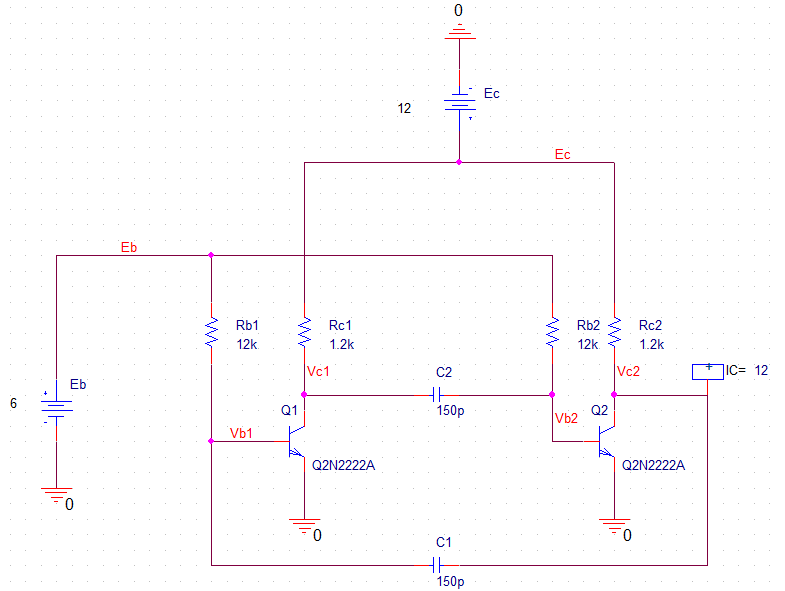
\includegraphics[width=\linewidth]{../img/schematic_vco.png}

\subsection{Simulation}

Après une première simulation, on a une fréquence d’oscillation de 238 kHz, ce qui n’entre pas dans les 2\% des 250kHz voulus, mais on pourra jouer sur $E_B$ plus tard avec un potentiomètre, et on pourrait également essayer d’autres valeurs pour les capacités avec les valeurs des résistances $R_B$ appairées.

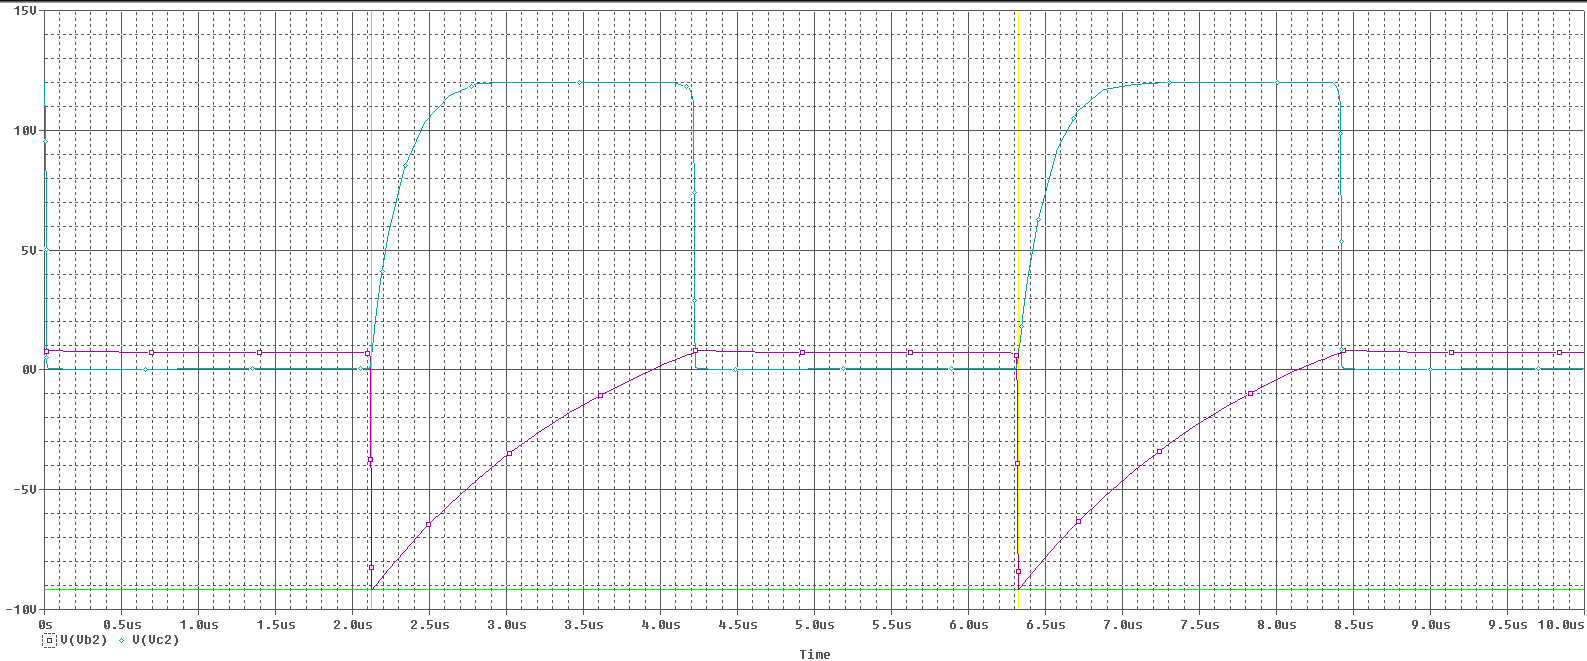
\includegraphics[width=\linewidth]{../img/oscillations_vco.png}

\subsection{Courbe de la fréquence en fonction de $E_B$}

$K = \cfrac{\Delta f}{\Delta v}$

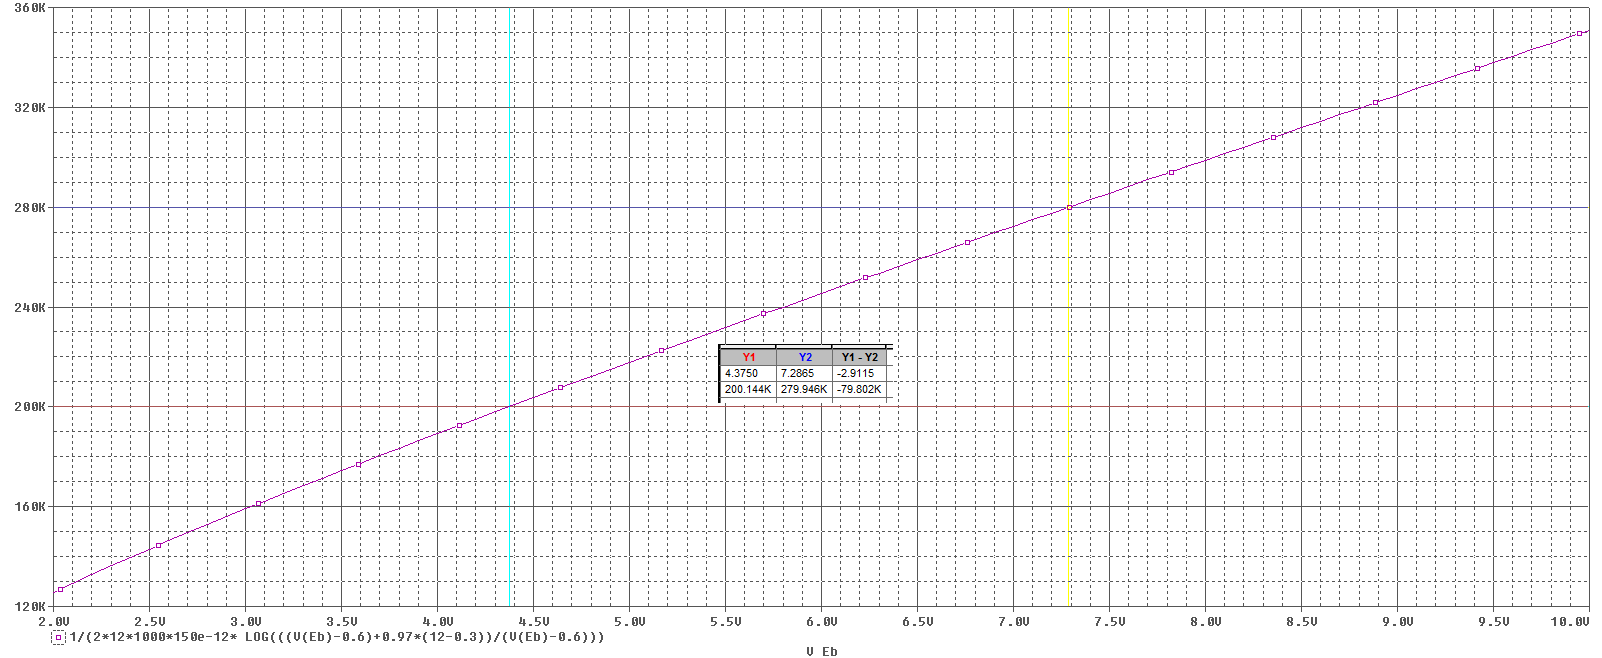
\includegraphics[width=\linewidth]{../img/variation_freq_vco.png}

\begin{minted}[linenos]{python}
Df2 = 79802
Dv2 = 2.9115
K = Df2/Dv2
\end{minted}
\verb|K = 27409.239223767814| \si{\Hz/\V}
\subsection{Analyse de Monte Carlo}

Pour chaque paramètre à étudier, on fait 500 simulations pour une distribution Gaussiene du paramètre, et on affiche un histograme des fréquences obtenues.
On devrait donc pouvoir comparer les 4 histogrammes obtenus pour voir rapidement quel paramètre a le plus d’influence.

Cependant, en regardant les équations, on s’attend à ce que les paramètres les plus influents sur la période soient R et C.

* On commence par regarder l’influence des paramètres R et C:

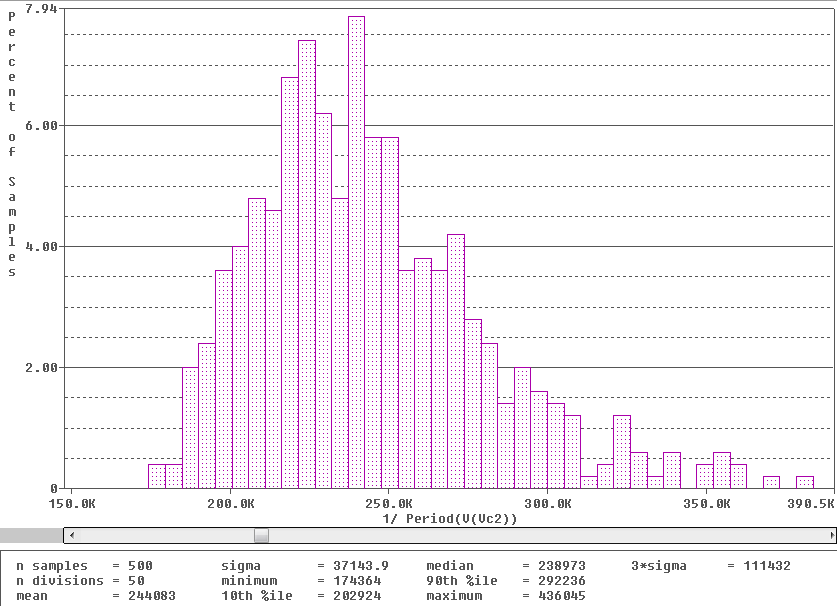
\includegraphics[width=\linewidth]{../img/montecarlo_R_C.png}


* Ensuite on regarde l’influence des paramètres du transistor, en commençant par $\beta$:

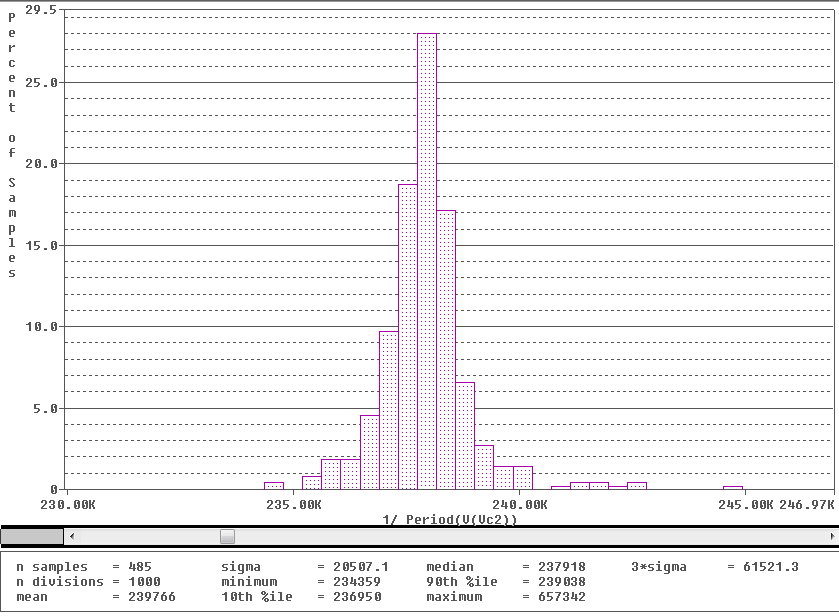
\includegraphics[width=\linewidth]{../img/montecarlo_beta.png}


On remarque que dans certains cas, la tension observée diverge, et spice nous en alerte.

* Puis $C_{jc}$:

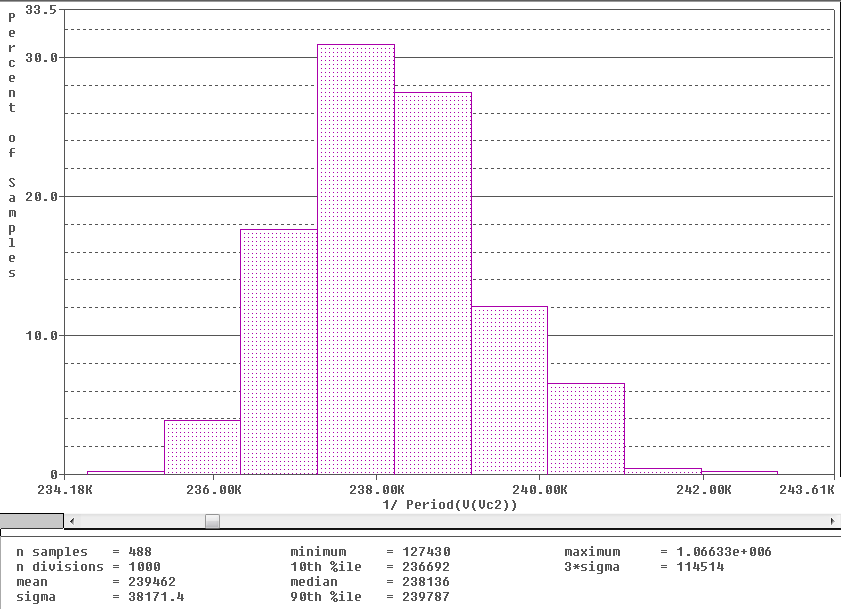
\includegraphics[width=\linewidth]{../img/montecarlo_Cjc.png}


* Et enfin $C_{je}$

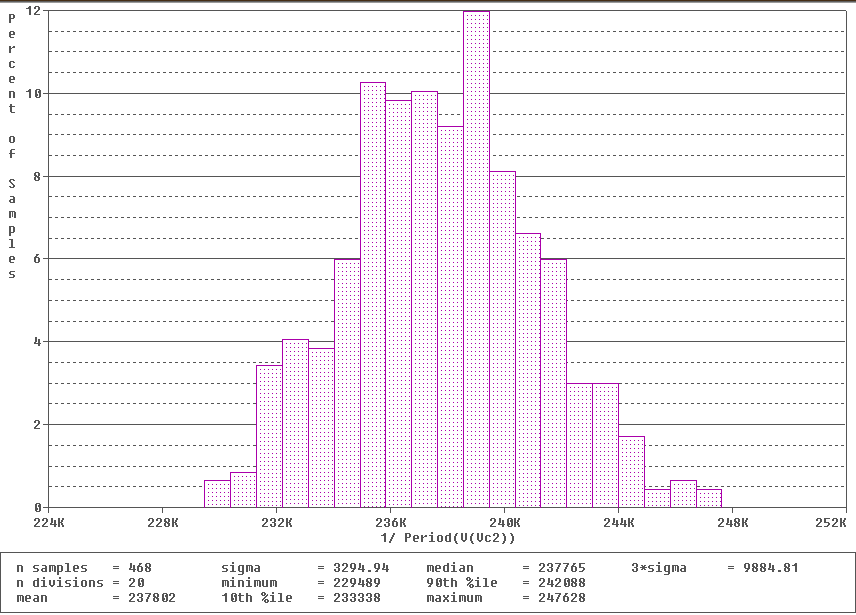
\includegraphics[width=\linewidth]{../img/montecarlo_Cje.png}


Comme on s’y attendait, les paramètres les plus influents sont de loins R et C.
En effet, une variation de ceux-ci modifie fait varier la fréquence d’une centaine de \si{\kilo\hertz}, alors que pour les autres c’est plutôt de l’ordre de 5 \si{\kilo\hertz}.
\subsection{Hiérarchisation du VCO}

En suivant le polycopié «Orcad-Pspice Hierarchie et sous-circuit», nous avons changé notre schématique en une véritable librairie, et la schématique peut maintenant se comporter comme n’importe quel autre composant dans une autre schématique.

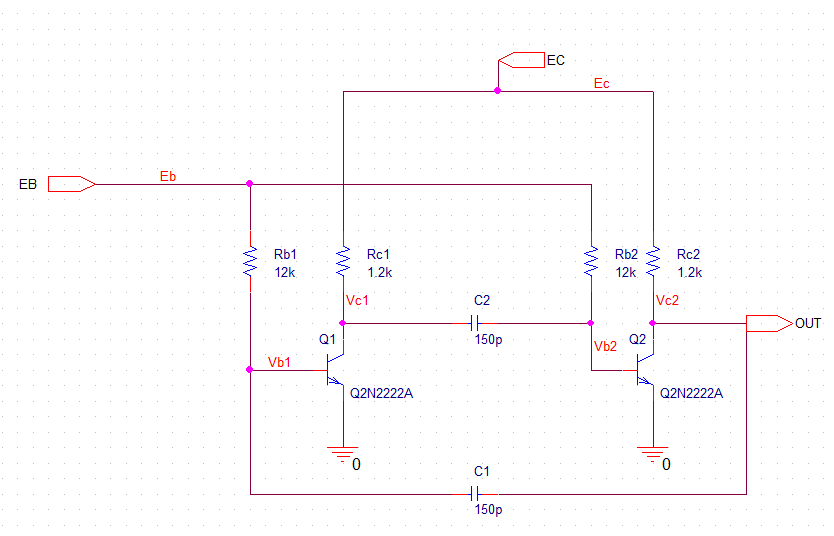
\includegraphics[width=\linewidth]{../img/schematic_low_hierarchy.png}


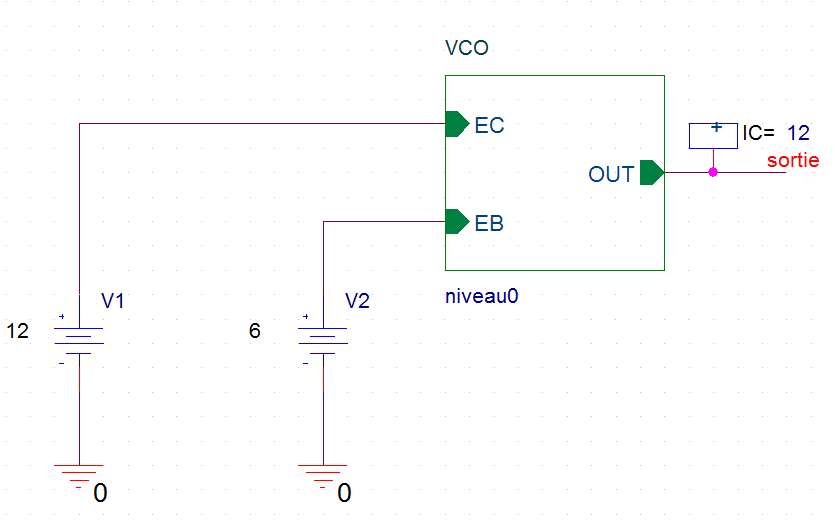
\includegraphics[width=\linewidth]{../img/schematic_high_hierarchy.png}


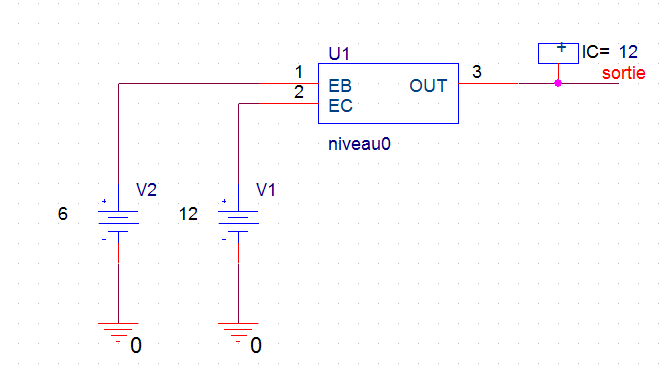
\includegraphics[width=\linewidth]{../img/schematic_vco_final.png}


On effectue enfine une simulation temporelle pour vérifier que tout continue de fonctionner:

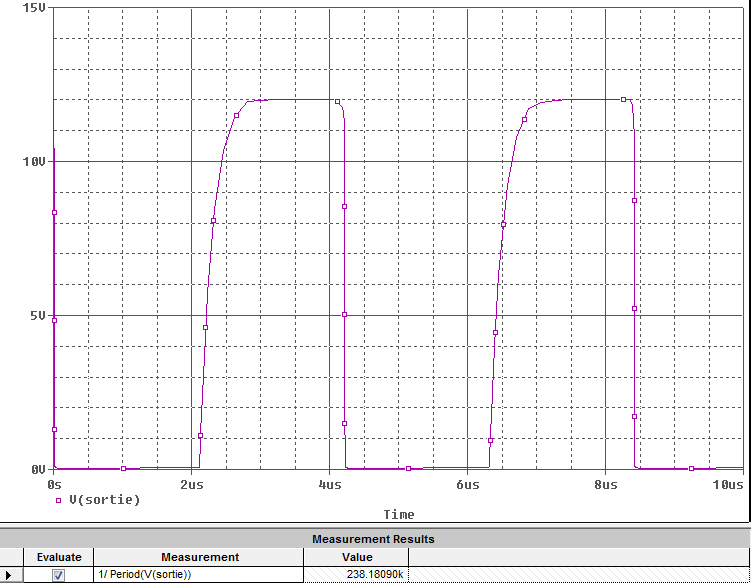
\includegraphics[width=\linewidth]{../img/simu_temporelle_bloc_hierarchique.png}

\subsection{Signal modulant BF}

On change enfin BC par un générateur sinusoïdal:

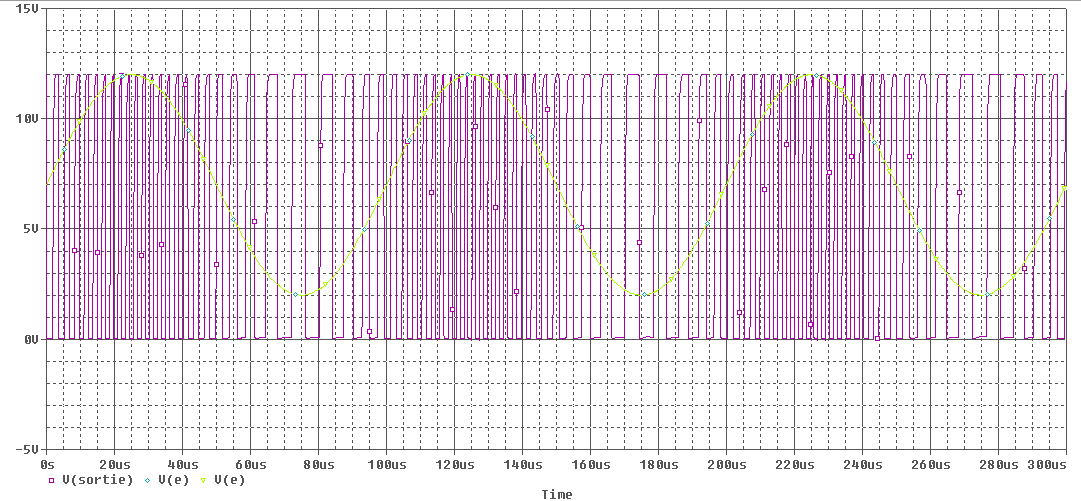
\includegraphics[width=\linewidth]{../img/variation_freq_sinus_en_entree.png}

Cette simulation montre bien que la fréquence du VCO varie avec la tension qu’on lui applique.

\section{Séance 2: Implémentation sur plaquette Labdec et mesures du VCO}
\subsection{Signal d’entrée de test}

Pour tester notre VCO, nous connectons son entrée à un potentiomètre suivi d’un amplificateur opérationnel suiveur, pour pouvoir faire varier la fréquence du VCO en modifant sa tension d’entrée via le potentiomètre.

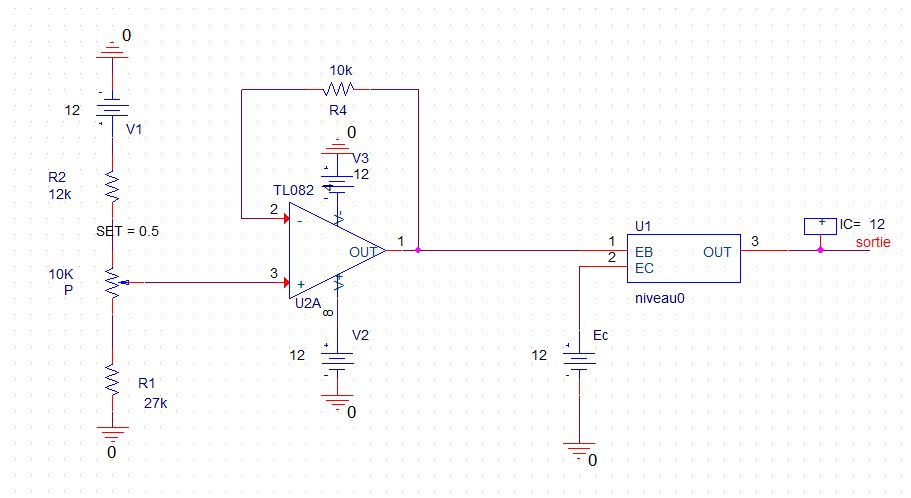
\includegraphics[width=\linewidth]{../img/schematic_test_vco.png}

\section{Séance 3: Simulation et mesures de l’amplificateur audio}

%TODO: Schéma p.54, bode théorique p.53

$G_0 = \cfrac{\Delta f}{K} = \cfrac{R_2}{R_1}\cfrac{R_5}{R_3}$

D’après le cahier des charges, $R_1 = 50 \si{\kilo\ohm}$ donc on prendra $R_1 = 47 \si{\kilo\ohm}$.

On a choisi à la séance précédente $R_5 = 10 \si{\kilo\ohm}$, donc pour simplifier les calculs, on prendra $\cfrac{R_5}{R_3} = 1 \Rightarrow R_3 = 10 \si{\kilo\ohm}$.

Il nous manque donc plus que $R_2$, qu’on détermine grace à $\Delta f = 15 kHz$ et $K = 26.5 kHz$.

Donc $R_2 = 27 \si{\kilo\ohm}$. De plus, $f_2 = 6 kHz \Rightarrow C_2 = \cfrac{1}{f_2 2 \pi 27000} = 1 nF$.

($f_2 = \cfrac{1}{2\pi R_4 C_4}$ \& $f_1 = \cfrac{1}{2\pi C_4(R_3 + R_4}$ ) $\Rightarrow$ ($C_4 = 17 nF \simeq 18nF$ \& $R_4 = 1473 Ohm \simeq 1.5 \si{\kilo\ohm}$).

$f_3 = f_4 = f_{CBF}\sqrt{\sqrt{2}-1} = 32 Hz$.

$f_3 = \cfrac{1}{2\pi C_3R_3} \Rightarrow C_3 = \cfrac{1}{32 \cdot 2 \pi \cdot 10000} = 500nF \simeq 470 nF$.

$f_4 = \cfrac{1}{2\pi C_1 (R_gR_1)} \simeq \cfrac{1}{2\pi R_1C_1} \Rightarrow C_1 = \cfrac{1}{32 \cdot 2 \pi \cdot 47000} = 100nF$.
\section{Séance 4: Simulation et mesures du circuit DEL}
\subsection{I − Circuits commutés}

$V_F=1.8V$

$I_0=100mA$

$R_{SC}\simeq 2Ohm$

$V_{CE_{sat}}=R_{SC}I_0=0.2V$

$E=R_6I_0+V_F+V_{CE_{sat}}\Rightarrow R6=\cfrac{E-V_F-V_{CE_{sat}}}{I_0}=100Ohm$
\begin{minted}[linenos]{python}
E = Quantity(12, V)
Vf = Quantity(1.8, V)
I0 = Quantity(0.1, A)
Rsc = Quantity(2, ohm)
Vcesat = Rsc * I0
\end{minted}
\verb|Vcesat = 200| \si{\milli\volt}
\begin{minted}[linenos]{python}
R6 = ( E - Vf - Vcesat) / I0
\end{minted}
\verb|R6 = 100| \si\ohm

$P_6=\cfrac{R_6I_0^2}{2}=0.5W$
\begin{minted}[linenos]{python}
P6 = R6 * I0**2 / 2
\end{minted}
\verb|P6 = 500| \si{\milli\watt}

$V_{E5}\simeq E-V_T$

$I_{B6}\simeq I_{C5}=\cfrac{V_{E5}}{R_{E5}}$

$R_{B6}=\cfrac{V_{E5}-V_{BE6}}{I_{B6}}=\cfrac{E-2V_T}{I_{B6}}$

On cherche a obtenir $I_{B6}$ supérieur à $\cfrac{I_0}{\beta}$ ; donc $R_{E5}\simeq R_{B6}\simeq 10\si{\kilo\ohm}$ font l’affaire.
\begin{minted}[linenos]{python}
Re5 = Quantity(10, 'kohm')
Ve5 = E-Vt
\end{minted}
\verb|Re5 = 10| \si{\kilo\ohm}
\begin{minted}[linenos]{python}
Rb6 = Re5 * (Ve5 - Vt) / Ve5
\end{minted}
\verb|Rb6 = 9.474| \si{\kilo\ohm}
\begin{minted}[linenos]{python}
Rb6 = Quantity(10, 'kohm')
\end{minted}
\begin{minted}[linenos]{python}
Ic5 = Ve5 / Re5
\end{minted}
\verb|Ic5 = 1.14| \si{\milli\ampere}

$R_{C5}\simeq\cfrac{V_T-V_{CE5}}{I_{C5}}$

Si on prend $V_{CE5} = 0.3V$, faible mais supérieur à $V_{CE_{sat}}=0.2V$, on obtient $R_{C5}=263 Ohm \simeq 270 Ohm$
\begin{minted}[linenos]{python}
Vce5 = Quantity(0.3, V)
Rc5 = (Vt - Vce5) / Ic5
\end{minted}
\verb|Rc5 = 263.158| \si\ohm
\subsection{III − Réduction des temps de montée}
\subsubsection{1 − Réduction de $t_{ri}$}

$C_6 > \cfrac{\beta}{2\pi f_TR_{B6}}$
\begin{minted}[linenos]{python}
fT = Quantity(250, 'kHz')
C6 = 100 / (Rb6 * 2 * pi * fT)
\end{minted}
\verb|C6 = 6.366| \si{\nano\farad}

On prend alors 100 \si{\nano\farad}.
\section{Séance 5: Routage de l’émetteur, dépôt du typon}
Ce routage s’est déroulé sans problème, voici à quoi ressemble notre typon:

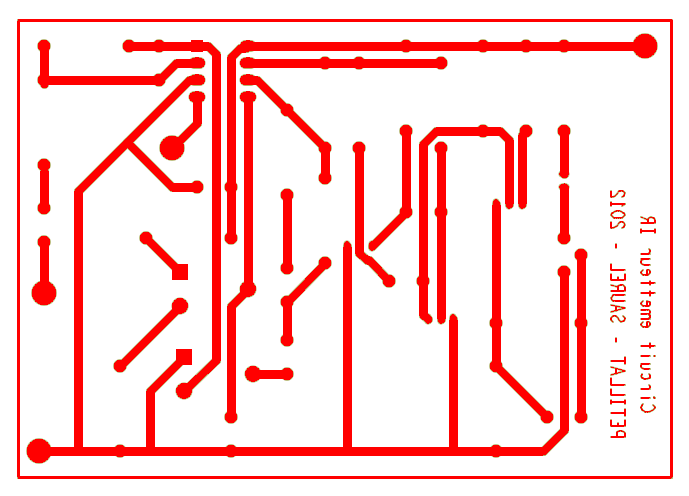
\includegraphics[width=\linewidth]{../img/routage.png}

\section{Séance 6: Soudage de la carte de l’émetteur − mesures de l’ḿetteur complet}
Cette séance mérite assez peu de commentaires techniques, si ce n’est «Ça marche».

Par contre, on peut ajouter qu’on est particulièrement content que ça marche aussi bien.



\end{document}

